%%%%%%%%%%%%%%%%%%%%%%%%%%%%%%%%%%%%%%%%%%%
	\begin{frame}{Historia}
		\begin{center}
			\movie[width=9.1cm,%
				height=5.2cm,%
				showcontrols=true,%
				loop,poster]{}{BrownianMotion.flv}
			\end{center}
		\end{frame}
%%%%%%%%%%%%%%%%%%%%%%%%%%%%%%%%%%%%%%%%%%%
\begin{frame}{Caminata del borracho}
	\centering
	\begin{tikzpicture}[
    ,
    axis/.style={thick, ->, >=stealth'},
    pile/.style={%
    	line width=1.0mm,
        ->, 
        >=stealth', 
        color = black!45!green
    	},
    every node/.style={%
    	color=black!40!blue
	   }
    ]
    % axis
    \draw[step=1cm,gray,very thin] (-1,-1) grid (6,6);
    \draw[axis] (-1,0)  -- (6,0) node(xline)[right]
        {$t$};
    \draw[axis] (0,-1) -- (0,6) node(yline)[above] {$X$};
    % Lines
    \draw[pile] (0,0) coordinate (A) -- (0,1)
        coordinate (B) node[right, text width=10em] {$\P[X_n=\pm 1]=1/2$};
    \draw[pile] (0,0) coordinate (C) -- (1,0)
        coordinate (D) node[below, text width=4em] {1}; 
	\end{tikzpicture}
\end{frame}
%%%%%%%%%%%%%%%%%%%%%%%%%%%%%%%%%%%%%%%%%%
\begin{frame}{Caminata Aleatoria}
	\begin{overlayarea}{\textwidth}{.7\textheight}
	\only<1>{
	\begin{center}
		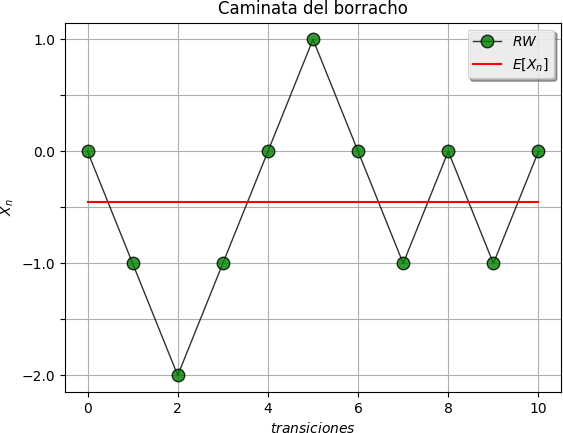
\includegraphics[width=.9\textwidth]{./IMAGENES/RW/RandomWalk_1_.png}
	\end{center}
	}
	\only<2>{
		\begin{center}
			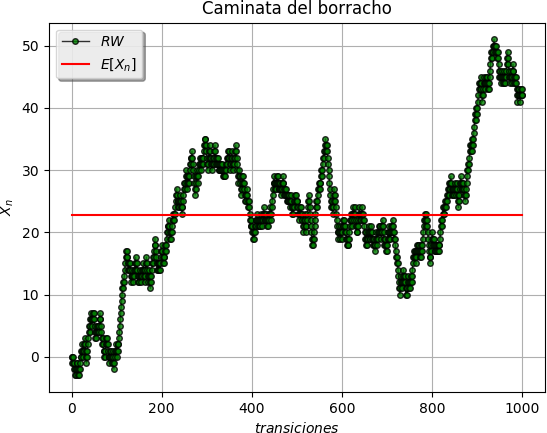
\includegraphics[width=0.83\textwidth]{./IMAGENES/RW/RandomWalk_2_.png}
		\end{center}
	}
	\only<3>{
		\begin{center}
			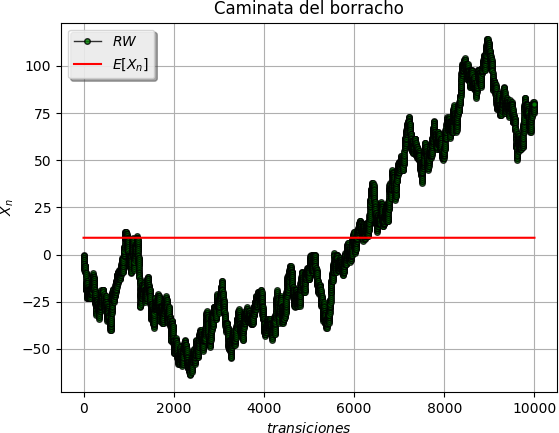
\includegraphics[width=0.83\textwidth]{./IMAGENES/RW/RandomWalk_3_.png}
		\end{center}
	}
	\end{overlayarea}
\end{frame}
%%%%%%%%%%%%%%%%%%%%%%%%%%%%%%%%%%%%%%%%%%%%%%%%%%%%%%%%%%%%%%%%%%%%%%%%%%%%%%%%
%%%%%%%%%%%%%%%%%%%%%%%%%%%%%%%%%%%%%%%%%%%%%%%%%%%%%%%%%%%%%%%%%%%%%%%%%%%%%%%%
\begin{frame}{Caminata del borracho}
	\centering
	\begin{tikzpicture}[
    scale=1,
    axis/.style={thick, ->, >=stealth'},
    pile/.style={%
    	line width=1.0mm,
        ->, 
        >=stealth', 
        color=black!45!green
    	},
    every node/.style={%
    	color=black!40!blue
	   }
    ]
    \draw[step=1cm,gray,very thin] (-1,-1) grid (6,6);
    \draw[axis] (-1,0)  -- (6,0) node(xline)[right]
        {$t$};
    \draw[axis] (0,-1) -- (0,6) node(yline)[above] {$Y_n$};
    \draw[pile] (0,0) coordinate (A) -- (0,1)
        coordinate (B) node[right, text width=10em] {%
        $\P[X_n=\pm \varepsilon]=1/2$%
        };%
    \draw[pile] (0,0) coordinate (C) -- (1,0)
        coordinate (D) node[below, text width=4em] {$\delta$}; 
	\end{tikzpicture}
\end{frame}
%%%%%%%%%%%%%%%%%%%%%%%%%%%%%%%%%%%%%%%%%%%%%%%%%%%%%%%%%%%%%%%%%%%%%%%%%%%%%%%
\begin{frame}{Construcci\'on}
	\begin{columns}
		\column[t]{.5\textwidth}
		\begin{overlayarea}{\textwidth}{\textheight}
			\only<2->{
				\begin{empheq}{align*}
					&\{ X_{n} \}_{n=1}^{\infty}   \quad v.a. .i.d\\
					&P(X_{j} = \pm \varepsilon)= \frac{1}{2}.
				\end{empheq}
			}
			\only<3->{
				\begin{empheq}[box=\shadowbox*]{align*}
					Y_{\delta, \varepsilon}(0) = &0\\
					Y_{ \delta, \varepsilon}(n \delta )= 
					&
					X_{1} + X_{2} + \cdots + X_{n}.
				\end{empheq}
			}
			\only<4->{
				Interpola linealmente
				\begin{empheq}{align*}
					Y_{\delta, \varepsilon}(t) =
						&
							\frac{(n + 1) \delta - t}{\delta} 
							Y_{\delta, \varepsilon} (n \delta)
						\\
					 +
					 &
						 \frac{t - n \delta}{\delta}
						 Y_{\delta, \varepsilon}
						\left(
							 (n+1) \delta
						\right).
					\\
					&
						n \delta < t < (n + 1) \delta .
				\end{empheq}
				}			
		\end{overlayarea}
	\column[t]{.6\textwidth}
		\begin{overlayarea}{\textwidth}{\textheight}
			\only<5->{
				\begin{alertblock}{Queremos}
					 $$
						\lim_{
							\substack{
								\delta\to 0\\
								\varepsilon \to 0
							}
						}
					 	Y_{\delta, \varepsilon}
					 $$
				\end{alertblock}
			}
			\only<6>{
				Tomate
		 		$
					\lambda \in \mathbb{R}
				$ fijo. Calcula
		 		\\
		 		\hyperlink{dfn:FuncionCaracteristica}{\beamergotobutton{caracteristica}}
				$
					\displaystyle
					\lim_{\delta, \varepsilon \to 0}
					\mathbb{E}
					\left[
						e^{ 
							i \lambda 
							Y_{\delta, \varepsilon}(t)
						}
					\right]
				$.
				\\
				\hypertarget{cns:Limite}{}
			}
			\only<7->{
				\textcolor<7>{red}{$t=n\delta$},
			}
			\only<7>{
				\begin{align*}
					\EX{
						e^{
							i\lambda
							Y_{\delta, \varepsilon}(\textcolor{red}{t})
						}
					}
					&=
					\prod_{j=1}^{n}
					\EX{
						e^{%
							i \lambda X_{j}%
						}
					}
					\\
					&=
					\left( 
						\EX{
							e^{i\lambda X_{j}}
						}
					\right)^{n}
					\\
					&=
					\left(
						\frac{1}{2} 
							e^{i \lambda \varepsilon}
					+
						\frac{1}{2}
							e^{-i \lambda \varepsilon}
					\right)^{n}
					\\
					&=
					\left(
						\cos(\lambda h)
					\right)^{n}\\
					&=
					\left(
						\textcolor{blue}{\cos(\lambda h)}
					\right)^{
									\frac{t}{
										\textcolor{blue}{\delta}
									}
							}.
				\end{align*}
			}
			\only<8->{
				\textcolor{cyan}{
					$
						u =
						\left(
							cos(\lambda \varepsilon)
						\right)^{\frac{1}{\delta}}
					$
				}
			}
			\only<9-10>{
				$
					\ln(u)= \frac{1}{\delta} 
					\ln(cos(\lambda \varepsilon))
				$
				\\
				Para $x$ chirris!!!
				$
					\ln(1+x)\approx x 
				$
				\\
				Para $\varepsilon$ chirris!!!
				$
					\cos(\lambda \epsilon)
					\approx 
					1 - \frac{1}{2} \lambda^2 \varepsilon^2	
				$.
				Entonces
			}
			\only<11-12>{
				\begin{empheq}{align*}
					u \approx 
						& 
						e^{ 
							- \frac{1}{2\delta}
							\lambda^{2}
							\varepsilon^{2}
						}
					\\
					\EX{
						e^{ 
							i \lambda 
							Y_{\delta, \varepsilon}(t)
						}
					}
					\approx &
					e^{
						- \frac{1}{
								2
								\textcolor{red}{\delta}
						}
						 t\lambda^{2}
						\textcolor{red}{\varepsilon}^{2}
					}.
			\end{empheq}
			}
			\only<11->{
				\textcolor{red}{$\varepsilon^{2} = \delta$}
			}
			\only<11->{
				$$
					\displaystyle
					\lim_{
						\delta \to 0 
					}
					\EX{
						e^{
							i \lambda 
							Y_{\delta, \sqrt{\delta}} (t)
						}
					}
					= 
					e^{ 
						-\frac{1}{2} t 
						\lambda^{2}
					},
					\qquad \lambda \in \mathbb{R}.
				$$
			}				\only<12>{
		 			\begin{empheq}[box=\ovalbox]{equation*}
		 			\therefore
		 			B(t)
		     			\overset{ \mathcal{D} }{ = }
		   				\displaystyle
		   				\lim_{\delta \to 0}
								Y_{\delta, \sqrt{\delta}}(t)
		 			\end{empheq}
				}
			\end{overlayarea}
		\end{columns}
	
\end{frame}
%%%%%%%%%%%%%%%%%%%%%%%%%%%%%%%%%%%%%%%%%%%%%%%%%%%%%%%%%%%%%%%%%%%%%%%%%%%%%%%
\begin{frame}{Construcci\'on}
	\begin{Teorema}
		Sea $Y_{\delta, \varepsilon}(t)$ una caminata aleatoria que inicia en $0$
		de saltos $\varepsilon$ y $-\varepsilon$  
		con igual probabilidad en los tiempos
		$\delta, 2\delta,3\delta, \ldots $.
		Supongamos que $\varepsilon^{2} = \delta$.
		Entonces para cada $t \geq 0$, el limite
		$$ 
			B(t) = \displaystyle
			\lim_{\delta \to 0}
			Y_{\delta, \sqrt{\delta}}(t),
		$$
		existe en distribución. Además, 
		$$
			\mathbb{E}\left[e^{i\lambda B(t)}\right]
				= e^{- \frac{1}{2}t\lambda^{2}}, \quad \quad \lambda \in 	\mathbb{R}.
		$$
	\end{Teorema}
\end{frame}
%%%%%%%%%%%%%%%%%%%%%%%%%%%%%%%%%%%%%%%%%%%%%%%%%%
\begin{frame}{Código}
	\only<+>{
  	\begin{figure}
  	\centering
      \tiny
   	\lstset{language=python}
         \lstinputlisting[firstline=3,lastline=11]{RW01.py}
   \end{figure}
}
\end{frame}
%%%%%%%%%%%%%%%%%%%%%%%%%%%%%%%%%%%%%%%%%%%
\begin{frame}{Caminata Aleatoria de $n$  transiciones}
	\begin{overlayarea}{\textwidth}{.7\textheight}
	\only<1>{
		\begin{center}
			\includegraphics[width=.85\textwidth,keepaspectratio]%
			{./IMAGENES/RW/RW01_1_.png}
		\end{center}
	}
	\only<2>{
		\begin{center}
			\includegraphics[width=.85\textwidth,keepaspectratio]%
			{./IMAGENES/RW/RW01_2_.png}
		\end{center}
	}
	\only<3>{
		\begin{center}
			\includegraphics[width=.85\textwidth,keepaspectratio]%
			{./IMAGENES/RW/RW01_3_.png}
		\end{center}
	}
	\end{overlayarea}
\end{frame}
%%%%%%%%%%%%%%%%%%%%%%%%%%%%%%%%%%%%%%%%%%%%%%%%%%%%%%%%%%%%%%%%%%%%%%%%%
\begin{frame}{Construcci\'on}
	\begin{empheq}[box={\Garybox[Construcci\'on]}]{align*}
		\varepsilon^{2} 
		& =
			\delta
		\\
		Y_{\delta, \varepsilon}(t)
		& 
			\xrightarrow[\delta, \varepsilon \to 0]{%
				\mathcal{D}
			} B(t) 
			\qquad \forall t 
			\geq 0
			\\
		\EX{
			e^{i\lambda B(t)}
		}
		&
		\xrightarrow{\delta ,\varepsilon \to 0}
			e^{
				-\frac{1}{2}t
				\lambda^{2}
			}, \quad \lambda \in 	\mathbb{R}.
	\end{empheq}
\end{frame}
%%%%%%%%%%%%%%%%%%%%%%%%%%%%%%%%%%%%%%%%%%%%%%%%%%
\begin{frame}{Distribuci\'on Gaussiana}
	\begin{figure}
		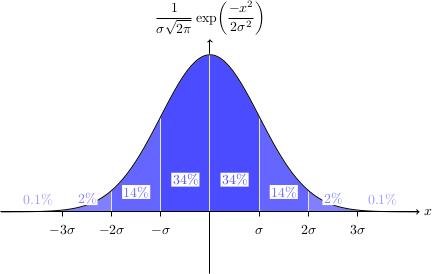
\includegraphics[width=\textwidth]{%
			./IMAGENES/RW/Standard_deviation_diagram.png%
		}
	\end{figure}
\end{frame}
%%%%%%%%%%%%%%%%%%%%%%%%%%%%%%%%%%%%%%%%%%%%%%%%%%%%%%%%%%%%%%%%%%%%%%%%%%
\begin{frame}{Caminata Aleatoria en $[0,1]$}
	%\vspace{-1.5cm}
	\begin{overlayarea}{\textwidth}{.7\textheight}
	\only<1>{
		\begin{center}
			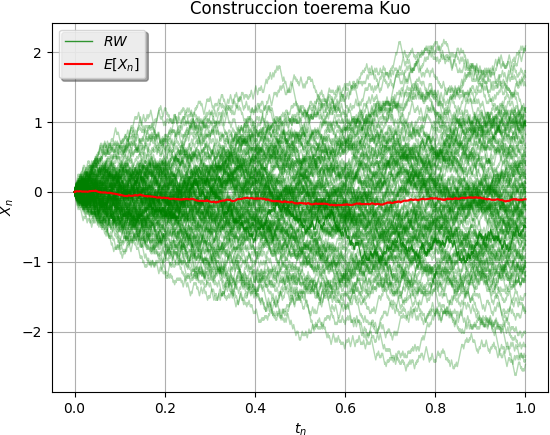
\includegraphics[width=.8\textwidth]{./IMAGENES/RW/RWs01.png}
		\end{center}
	}
	\only<2>{
		\begin{center}
			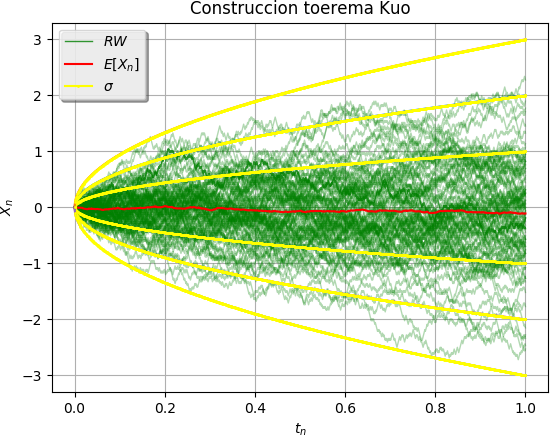
\includegraphics[width=.8\textwidth]{./IMAGENES/RW/RWs01Sigma.png}
		\end{center}
	}
	\end{overlayarea}
\end{frame}
%%%%%%%%%%%%%%%%%%%%%%%%%%%%%%%%%%%%%%%%%%%%%%%%%%%%%%%%%%%%%%%%%%%%%%%%%%%%%%%
\begin{frame}{Aproximación del MB en sentido Fuerte}
	\begin{definicion}
		El movimiento Browniano B(t) es el único proceso que satisface:
		\begin{enumerate}[(i)]
			\item 
				$B(0)=0$ c.s.
			\item 
				\textcolor<6>{orange}{
					Para $0\leq s \leq t$,
					$
						B(t) - B(s) \sim \sqrt{t-s} N(0,1).
					$
				}
			\item
				Para culquier $t_0 \leq t_1 \leq \dots \leq t_n \in [0,T]$, 
				las v.a
				$B(t_i)- B(t_j)$  son independientes 
		\end{enumerate}
	\end{definicion}
	\begin{overlayarea}{\textwidth}{0.5\textheight}
		\only<2-4>{
			Entonces, dados $t\in[0,T]$, y un stencil
			$$
				0=t_0\leq t_1 \leq \cdots \leq t_{M-1} \leq t_{M}=t
			$$
			\only<3>{
				$$
					B(t) = \sum_{j=1}^M 
						B(t_j)-B(t_{j-1}).
				$$
			}
			\only<4>{
			$$
				B(t) = \sum_{j=1}^M 
					\underbrace{
						B(t_j)-B(t_{j-1}).
					}_{:=\Delta B_j}
			$$
			}
		}
		\only<5-6>{
			Tomando $\{t_n\}_{n=0}^N$, $t_n = nh$, entonces
			$$
				B(t_n) \approx 
					\sum_ {j=0}^n \Delta B_j, 
					\qquad
					\Delta B_0:=0,
					\qquad
					\only<6>{
						\textcolor{orange}{
							\Delta B_j \sim \sqrt{h} N(0,1).
						}
					}
			$$	
		}
	\end{overlayarea}
\end{frame}
%%%%%%%%%%%%%%%%%%%%%%%%%%%%%%%%%%%%%%%%%%%%%%%%%%%%%%%%%%%%%%%%%%%%%%%%%%%%%%%%
